\documentclass[a4paper,12pt,twoside]{article}
\usepackage{preamble}
\usepackage{amsmath, amssymb, amscd, amsthm, amsfonts}
\usepackage{tcolorbox}
\usepackage{hyperref}
\usepackage{subfigure}
\usepackage[titlepage,fancysections,pagenumber]{polytechnique}

\title{INF567 Project}
\subtitle{Zero-Forcing Beamforming for Visible Light Communication Systems}
\author{Gabriel Pereira de Carvalho}

\date{\today}

\begin{document}
	
	\maketitle
	
	\tableofcontents
	
	\newpage
	
	\section{Introduction}
	
	\begin{tcolorbox}
		The code, simulation results, presentation slides and this report can be found on \href{https://github.com/ArkhamKnightGPC/INF567-Project}{the project's Github page}.
	\end{tcolorbox}
	
	Today, the processing power of edge devices (embedded systems on the frontier between computer networks and the physical world) allows them to perform more and more tasks independently. The networks connecting these devices (Internet of Things or IoT) has experienced tremendous growth.
	
	However, the RF technologies used for these networks (Wi-Fi, 4G or 5G) are experiencing more and more congestion due to the limited bandwidth available to all devices sharing the medium. In the literature, this problem is called \textbf{Spectrum crunch}.
	
	The visible light spectrum used by Visible Light Communication(VLC) technologies is approximately 1000 times larger than the entire radio frequency spectrum. This means less congestion, less interference and speeds higher than what is achievable with radio frequencies. Lab tests have achieved data rates of up to 224 gigabits per second\cite{LiFi}.
	
	\begin{figure}[h!]
		\centering
		\includegraphics[scale = 0.65]{images/VLCscheme.PNG}
		\caption{Concept diagram of indoor VLC system \cite{Indonesia2017}}
	\end{figure}
	
	It is important to highlight that VLC systems are not intended to replace RF technologies. VLC systems are more efficient in indoor environments and are complementary to RF technologies. In this project, we consider an indoor VLC system where the Access Points are connected to an outside network and the LED lamps are used only for communication inside the indoor environment. This is the principle of a specific type of VLC technology, called Light Fidelity or LiFi.
	
	The messages are transmitted using rapid fluctuations in LED light intensity (so fast they are invisible to the human eye). This means that LED lamps in a VLC network can provide light and simultaneously transmit data.
	
	Since light cannot penetrate walls, it's much harder for potential hackers or unauthorized individuals to access a VLC network. However, if there are multiple users in the indoor environment, the fact that the light is broadcasting information openly to the entire room can be problematic. For example, if VLC is deployed in a public library or space, it can be just as vulnerable as an RF system.
	
	The goal of this project is to explore the \textbf{zero-forcing beamforming} technique proposed in \cite{Oxford2021} for Physical Layer Security(PLS) to prevent both active and passive eavesdropping on VLC systems and attempt to replicate their results.
	
	\begin{tcolorbox}
		\textbf{What is the difference between Active and Passive EDs ?}
		
		The active EDs are devices that are in direct communication with the access points. They may pretend to be legitimate user, or introduce interference in the channel to force the access points to (unknowingly) increase the intensity of the signal at their location. However, since they are active users on the network they can be identified, and so we know their exact position and can work on a specific strategy against them.
		
		But passive EDs are devices that do not interfere or communicate with the network. In a VLC system, it can be any device like a camera or a smartphone with a photodetector that records light intensity measures. If these devices can demodulate the signal, they can get confidential messages without any knowledge of the network.
		
	\end{tcolorbox}
	
	\section{Modelisation of Indoor VLC system}
	
	Ok, so now that we have defined our context, let's present the specific details on the modelisation of the VLC system we will be simulating. The choices here try to follow as much as possible the paper \cite{Oxford2021}. Later when defining the optimization problems, I did some simplifications on the mathematics or used some ready \textit{scipy} functions instead of the precise approximation methods suggested in the paper but I will point out these decisions when we get there.
	
	The modulation/demodulation scheme analysed in \cite{Oxford2021} and considered for this project is IM/DD where \textbf{IM} (intensity modulation) refers to the method of encoding information by varying the intensity of the light source, which is then detected by a receiver. And \textbf{DD} (direct detection) refers to the detection of the transmitted signal by directly measuring the intensity of the received light, typically using a photodiode, without needing to decode phase or frequency information.
	
	The important takeaway here is that \textbf{we are not interested in details of the encoding algorithms but only on the intensity of light that is provided by the AP and that is received by the detector in each device}.
	
	We consider an IM/DD MIMO VLC system with:
	\begin{itemize}
		\item multiple Access Points(APs);
		\item a single Authorized User(AU);
		\item multiple Active Eavesdropping Devices(AEDs);
		\item and multiple Passive Eavesdropping Devices (PEDs).
	\end{itemize}
	
	\begin{figure}[h!]
		\centering
		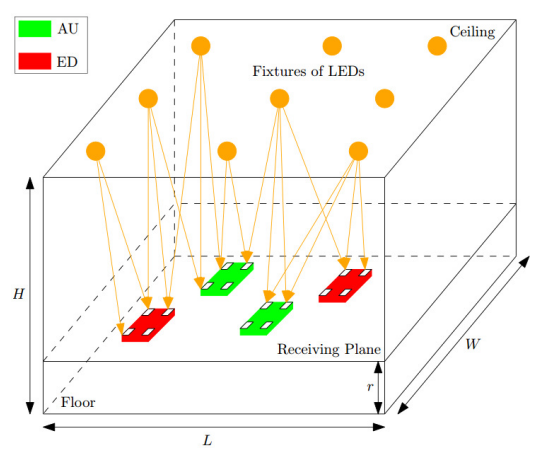
\includegraphics[scale=0.5]{../modelisation.PNG}
		\caption{Generalized model for MIMO VLC system \cite{Edinburgh2020}}
	\end{figure}
	
	As in \cite{Edinburgh2020}, we consider a room os size $L \times W \times H$. The room is equipped with $N$ APs that are located at its ceiling. The APs act as single transmitters, sending simultaneously a confidential message signal $s(t)$ to the AU in the presence of $P$ known AEDs $\{ AE_1, AE_2, ..., AE_P \}$ and $Q$ unknown randomly distributed PEDs $\{ PE_1, PE_2, ..., PE_Q \}$. We use the index $k \in \{AU, AE_p, PE_q\}$ to refer to a generic device.
	
	\section{Zero-Forcing Beamforming}
	
	Ideally, we want to maximize the SNR at the AU, and make it zero at every eavesdropping device. We can impose this constraint at the AEDs, whose position is known but it is more complicated to consider the PEDs whose position is unknown. We will discuss how to treat PEDs later in the report.
	
	Our goal is to determine the beamforming vector $w = [w_1,w_2,...,w_N]^T \in \mathbb{R}^N$ where $w_i$ is a weight for the signal from the $i$-th transmitter satisfying $\forall i \in \{1,2,...,N\}$:
	
	\begin{align}
		\begin{cases}
			w_i \in \mathbb{R} \\
			|w_i| \leq 1
		\end{cases}
	\end{align}
	
	Each AP will transmit a modulated signal $x_i(t)$. The LEDs are modelled as \textbf{Lambertian light sources}, which means that the observed luminous intensity is directly proportional to the cosine of the angle  $\psi_{i,k}$ between the observer's line of sight(\textbf{LoS}) and the surface normal
	\begin{equation}
		I = I_0 \cos( \psi_{i,k})
	\end{equation}
	this law is known as Lambert's emission law. We also define the angle of irradiance $\phi_{i,k}$ between the LoS and the surface normal at the AP.
	
	\begin{figure}[h!]
		\centering
		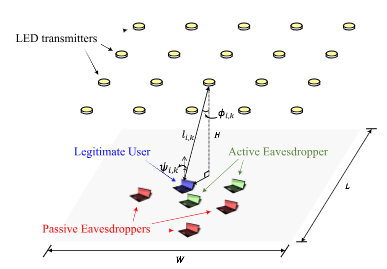
\includegraphics[scale=0.8]{../geometry.PNG}
		\caption{Geometrical parameters in the generalized VLC model \cite{Oxford2021}}
	\end{figure}
	
	For each device, we also introduce the channel gain vector $h_k = [h_{1,k}, h_{2,k}, ... , h_{N,k}]^T \in \mathbb{R}^N$ which models the effect of the channel on the signal during propagation. Reflections are ignored and only the direct path from source to receiver (LoS path) is considered. In \cite{Oxford2021} many physical constants are introduced, in the numerical simulation section most are taken as equal to $1$. To simplify the notation, let's omit these constants right from the start. We have
	\begin{equation}
		h_{i,k} = \cos(\phi_{i,k})\cos(\psi_{i,k})
	\end{equation}
	
	The modulated signal $x_i(t)$ is related to the message $s(t)$ by the relation
	\begin{equation}
		x_i(t) = \alpha I_{DC} s(t)
	\end{equation}
	where $\alpha \in [0, 1]$ is the modulation index and $I_{DC} \in \mathbb{R}_+$ is the current used by the AP LED for illumination. 
	
	By the superposition principle, the signal $y_k$ received at device $k$ is the sum of the signals received from each AP which gives
	\begin{equation}
		y_k(t) = \alpha I_DC (h_k \cdot w) s(t) + n_k(t)
	\end{equation}
	where $n_k(t)$ represents white Gaussian noise.
	
	Now that we now how to calculate the received signal at each point of the indoor environment, we can start defining the optimization problems we want to solve. In the paper \cite{Oxford2021}, he starts with multiple eavesdroppers and AEDs and PEDs right away, but I decided to start simpler and build the code from there. So first we look at the problem with one single AED, then we consider multiple AEDs and finally, we will see how to introduce the PEDs into our modelisation and how they affect the simulation results.
	
	We will also see that the number of access points has a big impact on the quality of the solutions. We will consider that the APs are distributed uniformly on an $N \times N$ grid on the ceiling of the room.
	
	\begin{figure}[h!]
		\centering
		\subfigure[]{
			\includegraphics[width=.4\textwidth]{../APgrid_N4.PNG}
		}
		\hfill
		\subfigure[]{
			\includegraphics[width=.4\textwidth]{../APgrid_N16.PNG}
		}
		\caption{Access point grids with $N=4$ and $N=16$}
		\label{APs}
	\end{figure}
	
	\newpage
	
	\section{Beamforming with one AED}
	
	Let's started with the traditional zero-forcing beamformer for a single AED $AE_1$, where the PEDs are ignored. The beamforming vector \( w \) must:
	\begin{enumerate}
		\item Maximize the received signal at the AU.
		\item Ensure that the signal received at the AED is zero.
	\end{enumerate}
	
	Here, we observe that (in linear algebra terms), since the received signal $y_k(t) = \alpha I_DC (h_k \cdot w) s(t) + n_k(t)$ is given by an inner product $(h_k \cdot w)$, to minimize the signal at the AED we need the beamforming vector $w$ to be perpendicular to the channel gain $h_k$ of the AED.
	
	The space $h_k^\perp$ (called the perpendicular complement of $h_k$) has dimension $N-1$, and any vector in this space will ensure that the signal received at the AED is zero. Now, to maximize the received signal at the AU, we project and normalize the channel chain $h_{AU}$ on $h_k^\perp$.
	
	\begin{figure}[h!]
		\centering
		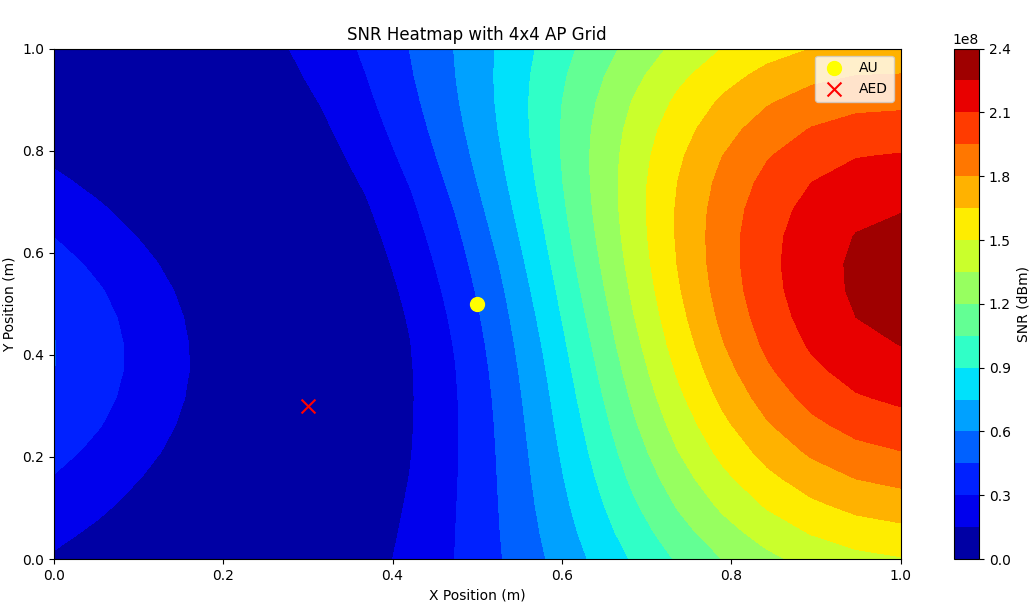
\includegraphics[width=.6\textwidth]{../oneAED.PNG}
		\caption{SNR simulation for zero-forcing beamforming with one AED}
	\end{figure}
	
	\newpage
	
	\section{Beamforming with multiple AEDs}
	
	When we consider $P>1$ AEDs, the received signals and channel gains now form matrices!
	
	\begin{equation}
		Y_{AED}(t) = \alpha I_DC (H_{AED} w) s(t) + N_{AED}(t) \quad \text{ with } H_{AED} =
		\begin{bmatrix}
			h_{AED_1}^T \\
			h_{AED_2}^T \\
			\vdots \\
			h_{AED_P}^T
		\end{bmatrix} 
	\end{equation}
	
	Now $H_{AED}$ defines a linear transformation on the beamforming vector $\implies$ to zero the signal at the AEDs, we need $w$ in the kernel(or null space) of $H_{AED}$. This can be computed with the \textit{scipy function} \href{https://docs.scipy.org/doc/scipy/reference/generated/scipy.linalg.null_space.html}{null\_space}.
	
	\begin{figure}[h!]
		\centering
		\subfigure[$N = 4$]{
			\includegraphics[width=.45\textwidth]{../multipleAED_N4.PNG}
		}
		\hfill
		\subfigure[$N = 16$]{
			\includegraphics[width=.45\textwidth]{../multipleAED_N16.PNG}
		}
		\caption{SNR simulation for zero-forcing beamforming with three AEDs}
	\end{figure}
	
	However, let's suppose that passive eavesdropping devices can be present in the room. We observe that in our solutions, the \textbf{peak SNR} is not at the authorized user but centered around some other point in the room. If a PED is present in this region, he will get a great quality of signal (better than the AU) and this represents a big security problem.
	
	We observe that this problem can be mitigated by increasing the number of access points. For $N=16$, the peak SNR is much smaller than for $N = 4$. In the paper\cite{Oxford2021}, the solution proposed is to add another constraint to the optimization problem.
	
	\section{Beamforming with multiple AEDs and possibility of PEDs}
	
	Since the PEDs can be uniformly distributed in the environment, the beamforming vector \( w \) must:
	\begin{enumerate}
		\item Maximize the received signal at the AU.
		\item Ensure that the signal received at the AED is zero.
		\item Ensure that the peak SNR is achieved at the AU (and not in another region where PEDs might be located).
	\end{enumerate}
	
	This is where the mathematics in the paper\cite{Oxford2021} gets complicated to generate precise solutions. I will propose an approximation that gave me very satisfying results. We will discretize the grid, similar to what we did with the APs to get a set of possible PED positions $\Omega$.
	
	\begin{figure}[h!]
		\centering
		\includegraphics[width=.5\textwidth]{../PEDgrid.PNG}
		\caption{Sampling of possible PED positions}
	\end{figure}
	
	Now, our optimization problem can be formulated as:
	\begin{align}
		\min_w \quad & \max_{(x,y) \in \Omega} \text{SNR}(x, y, w)  \\
		\text{s.t.} \quad & H_{AED} w = 0, \\
		& h_{AU} \cdot w = 1 \quad \text{ to ensure SNR is maximal at the AU}
	\end{align}
	
	This problem can be solved numerically using the \textit{scipy} \href{https://docs.scipy.org/doc/scipy/reference/generated/scipy.optimize.minimize.html}{minimize function} that offer different optimization methods. I have experimented with two different methods:
	\begin{itemize}
		\item \texttt{SLSQP} (Sequential Least Squares)
		\item \texttt{trust-constr} (Trust Region Constrained Algorithm)
	\end{itemize}
	The solutions generated were very similar, the difference being the computation time. The figure presented here was obtained with the \texttt{trust-constr} method. It is important to observe that computation time for the approximate solution rises very fast with the discretization resolution used to sample the PED positions, and with the number of access points used.
	
	\begin{figure}[h!]
		\centering
		\includegraphics[width=.6\textwidth]{../multipleAED_PED.PNG}
		\caption{SNR simulation for zero-forcing beamforming with two AED and possible PEDs}
	\end{figure}
	
	
	\begin{figure}[h!]
		\centering
		\includegraphics[width=.6\textwidth]{slides/simu2.PNG}
		\caption{SNR simulation for zero-forcing beamforming with four AED and possible PEDs}
	\end{figure}

	\begin{figure}[h!]
		\centering
		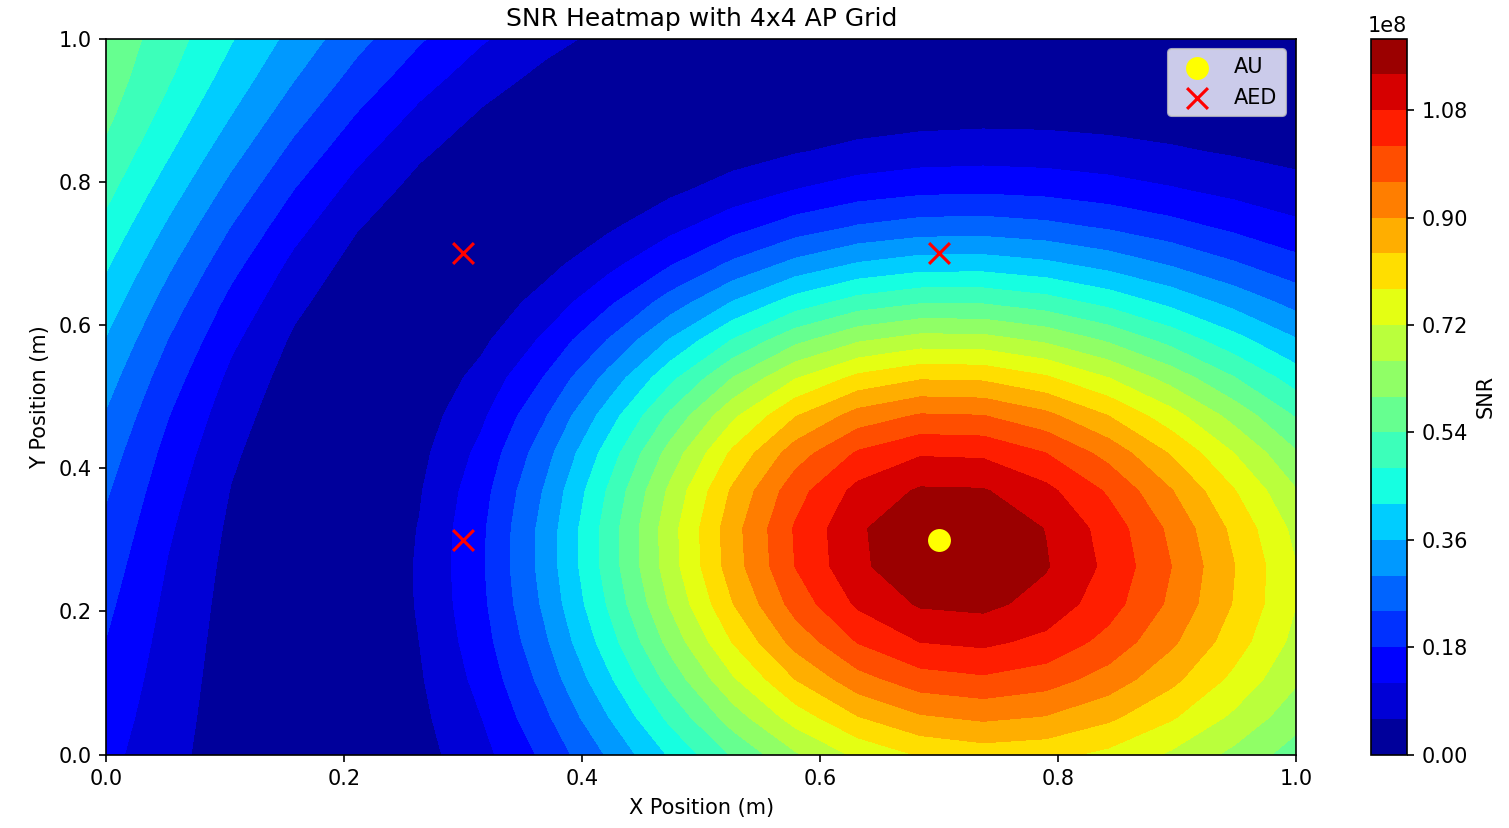
\includegraphics[width=.6\textwidth]{../simu3.PNG}
		\caption{SNR simulation for zero-forcing beamforming with three AED and possible PEDs}
	\end{figure}
	
	Comparing this SNR figure to one of the figures in the paper, we can see that the resolution achieved in the SNR figure was better with the more math-heavy method. But the approximated SNR figures are good solutions to the problem and manage to explore the tradeoffs we introduced when dealing with PEDs.
	
	\begin{figure}[h!]
		\centering
		\includegraphics[width=.6\textwidth]{../SNRpaper.PNG}
		\caption{SNR simulation from the paper\cite{Oxford2021}}
	\end{figure}

	\newpage
	
	\section{Conclusions}
	
	This project was a good introduction to Visible Light Communication systems in general, including topics such as Lifi and Physical Layer Security. Initially I wanted to make a physical prototype for a LiFi LED driver(ESP32 receiving text data over WiFi) and photoreceptor device(an Arduino UNO with an LDR for receiving the LED's signal and an LCD display to show the message received). However, to transmit and receive data using Manchester encoding, I ran into the problem of wireless clock synchronization. The whole interest of the project was to communicate with the Arduino without using the internet, but solving this clock synchronization problem is very hard without performing ping tests or access to an NTP(Network Time Protocol) server. There was also the issue of the LDR's speed which was slow compared to the LED and clock frequencies which made this synchronization over a preamble even harder. This could be solved with a faster and more sensitive photodetector like a photodiode.
	
	Ultimately, I decided to shift the focus of the project to a simulation based coding project. I am happy with the natural incremental development I was able to give to the zero-forcing beamforming techniques, gradually adding complexity to the problem. And I'm happy that I was able to get results relatively close to be complex SNR figures on the paper with a simpler approximation method. For future work on this project, there are some natural continuation points: implement the actual convex optimization method proposed on the paper, trying to relax the PED condition to simplify the problem and try to improve the quality/computation time of approximate solutions. Given that there are many recent publications on these beamforming techniques I'm sure it is an emerging topic with many active research problems.
	
	\newpage 

	\begin{thebibliography}{9}
		\bibitem{Edinburgh2020} Mohamed Amine Arfaoui, Mohammad Dehghani Soltani, Iman Tavakkolnia, Ali Ghrayeb, Majid Safari, Chadi M. Assi, Harald Haas (2020). \textbf{Physical Layer Security for Visible Light
		Communication Systems: A Survey}. IEEE Communications Surveys and Tutorials.
		
		\bibitem{Oxford2021}
		Sunghwan Cho, Gaojie Chen, Justin P. Coon (2021). \textbf{Zero-Forcing Beamforming for Active and Passive Eavesdropper Mitigation in Visible Light Communication Systems}. IEEE Transactions on Wireless Communications.
		
		\bibitem{Indonesia2017}
		E. Ramadhani, G.P. Mahardika (2017). \textbf{The Technology of Lifi: A Brief Introduction}. IOP Conference Series 2018.
		
		\bibitem{LiFi}
		LiFi.co. \textbf{LiFi Illuminated: Unleashing the Potential of Light-Based Connectivity} (Lifi white paper).
	\end{thebibliography}
	
\end{document}